\subsection{Resultados obtenidos por el prototipo a -10.00 C}

\begin{figure}[H]
	\centering
	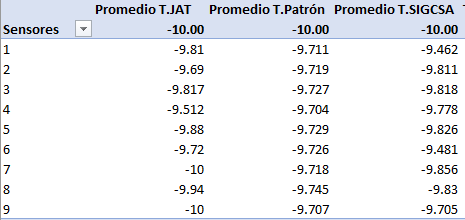
\includegraphics[width=0.5\linewidth]{resultados2.png}
	\caption{Tabla de Promedios de Temperaturas de prototipo y termómetros a -10.00 C}
\end{figure}

\par \noindent 
Los resultados de las pruebas son alentadores, en donde tomamos las 10 mediciones capturadas por el termómetro patrón, termómetro de campo de SIGCSA y nuestro prototipo, luego se procede a calcular sus respectivos promedios, ver figura 4.1. Con estos valores podemos realizar la siguiente gráfica:

\begin{figure}[H]
	\centering
	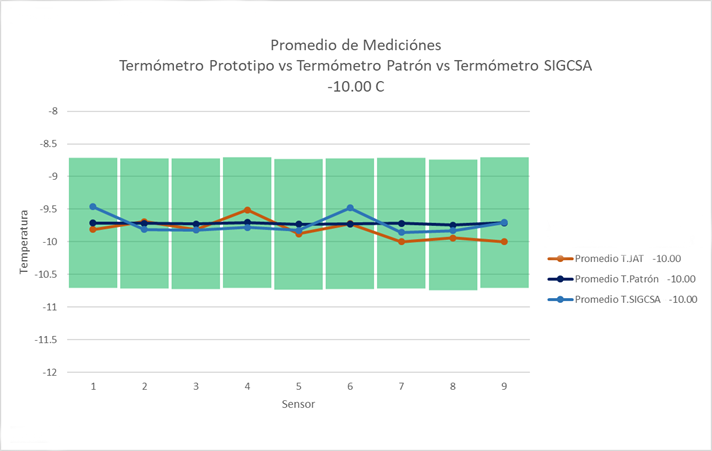
\includegraphics[width=0.6\linewidth]{resultados1.png}
	\caption{Gráfica de Promedios de Temperaturas de prototipo y termómetros a -10.00 C}
\end{figure}

\par \noindent
En la figura 4.2, podemos apreciar la línea del termómetro patrón con un color azul oscuro. Los termómetros de campo de SIGCSA con una línea azul claro y los sensores de nuestro prototipo en naranja oscuro. Como hemos utilizado el mismo termómetro patrón se pude notar que su línea es más uniforme. Las barras verdes representan el área en donde el termómetro de campo de SIGCSA y nuestro el sensor del prototipo se debe encontrar para cumplir con los estándares de la compañía. Tanto nuestro prototipo como el termómetro de campo cumplen. Se realizó el mismo procedimiento pero esta vez la temperatura a 0.00 C

